
\documentclass{jtetiproposalskripsi}

%-----------------------------------------------------------------
%Disini awal masukan untuk data proposal skripsi
%-----------------------------------------------------------------
\titleind{SISTEM PEMBELAJARAN MELALUI MEDIA ON-LINE 
(E-LEARNING) di UNIVERSITAS MUHAMMADIYAH JEMBER
}
\fullname{NUR LAILY KARTININGSIH}

\idnum{1200631014}

\approvaldate{14 Januari 2015}

\degree{Sarjana Komputer}

\yearsubmit{2015}

\program{Manajemen Informatika}

\headprogram{Sarjiya, S.T., M.T., Ph.D.}

\dept{Manajemen Informatika dan Teknik Informatika}

\firstsupervisor{Victor Wahanggara, S.Kom}
\firstnip{1203716}

\secondsupervisor{Mudafiq Ryan Pratama, S.Si}
\secondnip{1977 0131 2002 12 1 003}


%-----------------------------------------------------------------
%Disini akhir masukan untuk data proposal skripsi
%-----------------------------------------------------------------

\begin{document}

\cover

\approvalpage

%-----------------------------------------------------------------
%Disini akhir masukan untuk muka skripsi
%-----------------------------------------------------------------

%-----------------------------------------------------------------
%Disini awal masukan Intisari
%-----------------------------------------------------------------
\begin{abstractind}
Perkembangan teknologi informasi dan komunikasi pada saat ini sudah mengalami kemajuan yang sangat pesat. Media elektronik merupakan salah satu media yang diandalkan untuk mendapatkan informasi dan merupakan komunikasi. Internet adalah jaringan komputer global yang memanfaatkan salah satu media elektronik tercanggih (komputer) untuk memenuhi segala kebutuhan informasi dan komunikasi di segala bidang dengan akses yang cepat keseluruh dunia dengan biaya relative murah. Dengan memanfaatkan teknologi internet tersebut yang dapat diakses dalam jarak jauh dan waktu yang sangat cepat serta biaya yang relative murah, maka dunia pendidikan khususnya di Universitas Muhammadiyah Jember mulai menciptakan wahana baru dalam proses pembelajaran yaitu pembelajaran jarak jauh yang biasa di sebut dengan e-learning (elektronik  learning). Bagi institusi pendidikan, teknologi di dalam e-learning dapat dijadikan media untuk semakin memperbaiki kualitas dalam pembelajaran jarak jauh (distance learning). Untuk mengimbangi kemajuan teknologi informasi di era globalisasi dengan memberikan konsep yang berbeda dalam proses pembelajaran yang interaktif antara mahasiswa dengan dosennya. System pembelajaran melalui media on-line (e-learning) di Universitas Muhammadiyah Jember yang sekali dibahas secara mendetail yang disertai dengan pembahasan dan aplikasinya dengan menggunakan program Macromedia Dreamweaver dan AppServer.

\bigskip
\textbf{Kata kunci} : \emph{Sistem pembelajaran melalui media online , Macromedia Dreamweaver , AppServer}.
\end{abstractind}
%-----------------------------------------------------------------
%Disini akhir masukan Intisari
%-----------------------------------------------------------------

\tableofcontents
\addcontentsline{toc}{chapter}{DAFTAR ISI}
\selectlanguage{bahasa}\clearpage\pagenumbering{arabic}\setcounter{page}{1}

%-----------------------------------------------------------------
%Disini awal masukan untuk Bab
%-----------------------------------------------------------------
\chapter{LATAR BELAKANG}

\section{Latar Belakang Masalah}
Perkembangan teknologi informasi dan komunikasi pada saat ini sudah mengalami kemajuan yang sangat pesat. Media elektronik merupakan salah satu media yang diandalkan untuk mendapatkan informasi dan merupakan komunikasi. Internet adalah jaringan komputer global yang memanfaatkan salah satu media elektronik tercanggih (komputer) untuk memenuhi segala kebutuhan informasi dan komunikasi di segala bidang dengan akses yang cepat keseluruh dunia dengan biaya relative murah.

Dengan memanfaatkan teknologi internet tersebut yang dapat diakses dalam jarak jauh dan waktu yang sangat cepat serta biaya yang relative murah, maka dunia pendidikan khususnya di Universitas Muhammadiyah Jember mulai menciptakan wahana baru dalam proses pembelajaran yaitu pembelajaran jarak jauh yang biasa di sebut dengan e-learning (elektronik  learning). Bagi institusi pendidikan, teknologi di dalam e-learning dapat dijadikan media untuk semakin memperbaiki kualitas dalam pembelajaran jarak jauh (distance learning). Banyak yang menganggap bahwa e-learning terkesan sebagai pembelajaran yang pasif dan hanya satu arah dari staf pengajar semata, sedikit demi sedikit hal ini mulai terpecahkan. Dukungan multimedia yang semakin canggih dan perkembangan baru di dunia web semakin membantu mewujudkan pembelajaran interaktif, meskipun tidak harus bertemu langsung secara fisik.

Lembaga pendidikan dimanapun sangat memerlukan e-learning sebagai wahana  pembelajaran jarak jauh yang mudah diakses. Hal tersebut dapat kita manfaatkan dengan fasilitas internet dengan mempunyai website untuk menyediakan layanan akses kepada para mahasiswa dan komponen kampus yang membutuhkan informasi terkini sehingga lebih efektif dan efisien.
Untuk mengimbangi kemajuan teknologi informasi di era globalisasi dengan memberikan konsep yang berbeda dalam proses pembelajaran yang interaktif antara mahasiswa dengan dosennya. System pembelajaran melalui media on-line (e-learning) di Universitas Muhammadiyah Jember yang sekali dibahas secara mendetail yang disertai dengan pembahasan dan aplikasinya dengan menggunakan program Macromedia Dreamweaver dan AppServer.


\section{Perumusan Masalah}
\begin{itemize}
\item[1.]Bagaimana peranan e-learning dimata para mahasiswa pada proses pembelajaran ?
\item[2.]Apa Kekurangan dari proses pembelajaran melalui e-learning bagi para mahasiswa dan dosen?
\item[3.]Apa saja manfaat dari proses pembelajaran melalui e-learning bagi para mahasiswa dan dosen ?
\end{itemize}

\section{Batasan Masalah}
Dalam menggunakan media on-line di Universitas Muhammadiyah Jember khususnya dalam matakuliah Sistem Basis Data untuk mengajar para mahasiswa, bisa membantu mahasiswa untuk menyesuaikan pada perkembangan ilmu pengetahuan dan teknologi informasi serta situasi pendukung yang lain khususnya di matakuliah Sistem Basis Data tersebut.


\section{Tujuan Penelitian}
Adapun tujuan dari penelitian ini adalah :
\begin{itemize}
\item[1.]Untuk memberikan suatu alternative wacana peningkatan mutu pendidikan khususnya peningkatan hasil pembelajaran melalui E-learning.
\item[2.]Meningkatkan mutu pendidikan, dengan asumsi bahwa komputer adalah merupakan sesuatu yang wajib ada bagi universitas muhammadiyah jember sedangkan internet adalah sebagai suatu hal yang harus bisa di pahamin oleh mahasiswa.
\end{itemize}


\section{Manfaat Penelitian}
Manfaat dari dibuatnya sistem ini yaitu :
\begin{itemize}
\item[1.]Mahasiswa dapat berinteraksi dengan dosen nya sevara on-line di tempat yang berbeda.
\item[2.]Mahasiswa dapat mengetahui persiapan materi yang akan diterimanya untuk minggu-minggu kedepan.
\item[3.]Mahasiswa dapat mengukur dan mengevaluasi kemanpuanya secara on-line.
\item[4.]Memiliki tambahan pengetahuan atau wawasan bagi pengunjung e-learning.
\end{itemize}

%-------------------------------------------------------------------------------
\chapter{KAJIAN PUSTAKA}               
\section{Peranan e-learning dimata para mahasiswa pada proses pembelajaran.}
Penerapan e-learning yang efektif, menurut Indrayani (2007), berhubungan dengan usaha yang konsisten dan terintegrasi dari pelajar, lembaga, fasilitator, staff penunjang, dan administrator. Harrison (dalam Pushpanathan, 2012) menjelaskan bahwa guru berperan sebagai “pelajar ahli” yang dapat membantu siswa memecahkan masalah dan mencari jawaban dari pertanyaan-pertanyaan mereka. Proses pembelajaran berbasis e-learning akan lebih berhasil jika guru memenuhi ciri berikut:
\begin{itemize}
\item[1.]Memiliki semangat yang tinggi.
\item[2.]Dapat mengatur sesi belajar dengan baik.
\item[3.]Mencintai subjek yang diajarkan
\item[4.]Dapat mengkonseptualisasi topik yang dibahas
\item[5.]Berempati terhadap siswa
\item[6.]Memahami bagaimana cara manusia belajar
\item[7.]Memiliki keterampilan mengajar dan mengelola pembelajaran
\item[8.]Waspada terhadap tiap kejadian di dalam kelas
\item[9.]Mengajar dengan gaya pengajaran yang ia sukai
\item[10.]Terampil dalam berbagai aspek pengajaran: bertanya, mendengarkan, mendorong, bereaksi, menyimpulkan, dan memimpin.
\end{itemize}

Selain yang telah disebutkan di atas, untuk meningkatkan motivasi belajar dan memaksimalkan proses pembelajaran, setiap guru harus membekali diri dengan keterampilan TIK dan pengetahuan terkait teknologi yang cukup mumpuni. Pelgrum (dalam Khan dkk, 2012) menyatakan bahwa kurangnya keterampilan dan pengetahuan guru merupakan salah satu dari hambatan utama penggunaan internet dalam pembelajaran di negara yang sedang dan belum berkembang. Hal serupa diungkapkan Olowa (2012), yaitu bahwa di beberapa negara, prospek penggunaan internet untuk proses pembelajaran belum diterapkan secara maksimal dan masih terbatas. Keterbatasan tersebut terutama disebabkan oleh kurang mendukungnya fasilitas di sekolah, biaya penggunaan internet yang tinggi, dan kurangnya pengetahuan serta keterampilan guru dalam menggunakan internet untuk tujuan pembelajaran.

Perbedaan Pembelajaran Tradisional dengan e-learning, yaitu kelas ‘tradisional’, guru dianggap sebagai orang yang serba tahu dan ditugaskan untuk menyalurkan ilmu pengetahuan kepada pelajarnya. Sedangkan di dalam pembelajaran e-learning fokus utama adalah pelajar. Pelajar mandiri pada waktu tertentu dan bertanggung jawab untuk pembelajarannya. Suasana pembelajaran e-learning akan “memaksa” pelajar memainkan peranan yang lebih aktif dalam pembelajarannya. Pelajar membuat perancangan dan mencari materi dengan usaha dan inisiatif sendiri. E-Learning adalah pembelajaran jarak jauh (distance Learning) yang memanfaatkan teknologi komputer, jaringan komputer dan/atau Internet. E-Learning memungkinkan pembelajar untuk belajar melalui komputer di tempat mereka masing-masing tanpa harus secara fisik pergi mengikuti pelajaran/perkuliahan di kelas. E-Learning sering pula dipahami sebagai suatu bentuk pembelajaran berbasis web yang bisa diakses dari intranet di jaringan lokal atau internet.

Secara sederhana dapat dikatakan bahwa semua pembelajaran dilakukan dengan memanfaatkan teknologi internet dan selama proses belajar dirasakan terjadi oleh yang mengikutinya, maka kegiatan itu dapat disebut sebagai pembelajaran berbasis web. Dalam pendidikan, e-learning dapat diartikan pembelajaran yang dilaksanakan dengan memanfaatkan fungsi internet dalam kegiatan pembelajaran dengan menjadikan fasilitas elektronik sebagai media pembelajaran.

\section{Kekurangan dari proses pembelajaran melalui e-learning bagi para mahasiswa dan dosen}
Beberapa kekurangan yang dimiliki oleh pemanfaatan e-Learning :
\begin{itemize}
\item[1.]Kurangnya interaksi antara pengajar dan pelajar atau bahkan antar pelajar itu sendiri. Kurangnya interaksi ini bisa memperlambat terbentuknya values dalam proses belajar mengajar. Kecenderungan mengabaikan aspek akademik atau aspek sosial dan sebaliknya mendorong tumbuhnya aspek bisnis/komersial.
\item[2.]Proses belajar mengajar cenderung ke arah pelatihan daripada pendidikan.
\item[3.]Berubahnya peran pengajar dari yang semula menguasai teknik pembelajaran konvensional, kini juga dituntut mengetahui teknik pembelajaran yang menggunakan ICT (Information, Communication and Technology). Tidak semua tempat tersedia fasilitas internet ( mungkin hal ini berkaitan dengan masalah tersedianya listrik, telepon ataupun komputer).
\item[4.]Kurangnya mereka yang mengetahui dan memiliki keterampilan tentang internet.
\item[5.]Kurangnya interaksi antara guru dan siswa atau bahkan antar siswa itu sendiri sehingga memperlambat terbentuknya nilai dalam proses belajar dan mengajar.
\item[6.]Kurangnya penguasaan bahasa komputer.
\end{itemize}

\section{Manfaat dari proses pembelajaran melalui e-learning}
Manfaat pembelajaran melalui e–learning menurut A. W. Bates (Bates, 1995) dan K. Wulf (Wulf, 1996) terdiri atas 4 hal, yaitu:
\begin{itemize}
\item[1.]Meningkatkan kadar interaksi pembelajaran antara peserta didik dengan guru atau instruktur (enhance interactivity). Apabila dirancang secara cermat, pembelajaran elektronik dapat meningkatkan kadar interaksi pembelajaran, baik antara peserta didik dengan guru/instruktur, antara sesama peserta didik, maupun antara peserta didik dengan bahan belajar (enhance interactivity). Berbeda halnya dengan pembelajaran yang bersifat konvensional. Tidak semua peserta didik dalam kegiatan pembelajaran konvensional dapat, berani atau mempunyai kesempatan untuk mengajukan pertanyaan ataupun menyampaikan pendapatnya di dalam diskusi. Mengapa? Karena pada pembelajaran yang bersifat konvensional, kesempatan yang ada atau yang disediakan dosen/guru/instruktur untuk berdiskusi atau bertanya jawab sangat terbatas. Biasanya kesempatan yang terbatas ini juga cenderung didominasi oleh beberapa peserta didik yang cepat tanggap dan berani. Keadaan yang demikian ini tidak akan terjadi pada pembelajaran elektronik.Peserta didik yang malu maupun yang ragu-ragu atau kurang berani mempunyai peluang yang luas untuk mengajukan pertanyaan maupun menyampaikan pernyataan/pendapat tanpa merasa diawasi atau mendapat tekanan dari teman sekelas (Loftus, 2001). 
\item[2.]Memungkinkan terjadinya interaksi pembelajaran dari mana dan kapan saja (time and place flexibility). Mengingat sumber belajar yang sudah dikemas secara elektronik dan tersedia untuk diakses oleh peserta didik melalui internet, maka peserta didik dapat melakukan interaksi dengan sumber belajar ini kapan saja dan dari mana saja (Dowling, 2002). Demikian juga dengan tugas-tugas kegiatan pembelajaran, dapat diserahkan kepada instruktur begitu selesai dikerjakan. Tidak perlu menunggu sampai ada janji untuk bertemu dengan guru/instruktur. Peserta didik tidak terikat ketat dengan waktu dan tempat penyelenggaraan kegiatan pembelajaran sebagaimana halnya pada pendidikan konvensional. Dalam kaitan ini, Universitas Terbuka Inggris telah memanfaatkan internet sebagai metode/media penyajian materi. Sedangkan di Universitas Terbuka Indonesia (UT), penggunaan internet untuk kegiatan pembelajaran telah dikembangkan. Pada tahap awal, penggunaan internet di UT masih terbatas untuk kegiatan tutorial saja atau yang disebut sebagai “tutorial elektronik” (Anggoro, 2001).
\item[3.]Menjangkau peserta didik dalam cakupan yang luas (potential to reach a global audience). Dengan fleksibilitas waktu dan tempat, maka jumlah peserta didik yang dapat dijangkau melalui kegiatan pembelajaran elektronik semakin lebih banyak atau meluas. Ruang dan tempat serta waktu tidak lagi menjadi hambatan. Siapa saja, di mana saja, dan kapan saja, seseorang dapat belajar. Interaksi dengan sumber belajar dilakukan melalui internet. Kesempatan belajar benar-benar terbuka lebar bagi siapa saja yang membutuhkan.
\item[4.]Mempermudah penyempurnaan dan penyimpanan materi pembelajaran (easy updating of content as well as archivable capabilities). Fasilitas yang tersedia dalam teknologi internet dan berbagai perangkat lunak yang terus berkembang turut membantu mempermudah pengembangan bahan belajar elektronik. Demikian juga dengan penyempurnaan atau pemutakhiran bahan belajar sesuai dengan tuntutan perkembangan materi keilmuannya dapat dilakukan secara periodik dan mudah. Di samping itu, penyempurnaan metode penyajian materi pembelajaran dapat pula dilakukan, baik yang didasarkan atas umpan balik dari peserta didik maupun atas hasil penilaian instruktur selaku penanggung-jawab atau pembina materi pembelajaran itu sendiri. Pengetahuan dan keterampilan untuk pengembangan bahan belajar elektronik ini perlu dikuasai terlebih dahulu oleh instruktur yang akan mengembangkan bahan belajar elektronik. Demikian juga dengan pengelolaan kegiatan pembelajarannya sendiri. Harus ada komitmen dari instruktur yang akan memantau perkembangan kegiatan belajar peserta didiknya dan sekaligus secara teratur memotivasi peserta didiknya.

\item •Manfaat bagi siswa :
Dengan kegiatan e-Learning dimungkinkan berkembangnya fleksibilitas belajar yang tinggi. Artinya, kita dapat mengakses bahan-bahan belajar setiap saat dan berulang-ulang. Selain itu kita juga dapat berkomunikasi dengan guru/dosen setiap saat, misalnya melalui chatting dan email. Mengingat sumber belajar yang sudah dikemas secara elektronik dan tersedia untuk diakses melalui internet, maka kita dapat melakukan interaksi dengan sumber belajar ini kapan saja dan dari mana saja, juga tugas-tugas pekerjaan rumah dapat diserahkan kepada guru/dosen begitu selesai dikerjakan. 
\item •Manfaat bagi pengajar :
Dengan adanya kegiatan e-Learning manfaat yang diperoleh guru/dosen antara lain adalah bahwa guru/dosen/ instruktur akan lebih mudah melakukan pembaruan materi maupun model pengajaran sesuai dengan tuntutan perkembangan keilmuan yang terjadi, juga dapat dengan efisien mengontrol kegiatan belajar siswanya. 
\end{itemize}
Pengalaman negara lain dan juga pengalaman distance learning di Indonesia ternyata menunjukkan sukses yang signifikan, antara lain: 
\begin{itemize}
\item[a.] Mampu meningkatkan pemerataan pendidikan;
\item[b.] Mengurangi angka putus sekolah atau putus kuliah atau putus sekolah;
\item[c.] Meningkatkan prestasi belajar;
\item[d.] Meningkatkan kehadiran siswa di kelas,
\item[e.] Meningkatkan rasa percaya diri; 
\item[f.] Meningkatkan wawasan (outward looking); 
\item[g.] Mengatasi kekurangan tenaga pendidikan; serta 
\item[h.] Meningkatkan efisiensi. (Soekartawi, 2005)
\end{itemize}
Keuntungan menggunakan e-Learning diantaranya adalah sebagai berikut: 
\begin{itemize}
\item[a.] Menghemat waktu proses belajar mengajar 
\item[b.] Mengurangi biaya perjalanan 
\item[c.] Menghemat biaya pendidikan secara keseluruhan (infrastruktur, peralatan, buku-buku) 
\item[d.] Menjangkau wilayah geografis yang lebih luas 
\item[e.] Melatih pembelajar lebih mandiri dalam mendapatkan ilmu pengetahuan
\end{itemize}

%-------------------------------------------------------------------------------
\chapter{METODE PENELITIAN}

\section{Lokasi Penelitian}
Kegiatan penelitian ini dilakukan di kampus Universitas Muhammadiyah Jember Kabupaten Jember yang beralamat di Jl. Karimata No. 49.
Universitas Muhammadiyah Jember merupakan kampus yang pembelajarannya menggunakan media online (E-learning).

\section{Teknik Pengumpulan Data}
Teknik pengumpulan data disini menggunakan teknik wawancara digunakan untuk meyakinkan bahwa data yang diperoleh benar-benar akurat dan pada kesempatan ini penulis mewawancarai pada bagian mahasiswa dan dosen untuk mengetahui dan mencatat data-data yang diperlukan. 

\section{Tahapan Penelitian}
\begin{itemize}
\item[1.]Menentukan banyaknya mahasiswa Universitas Muhammadiyah Jember.
\item[2.]Mengadakan wawancara (interiew) dan dokumentasi untuk memperoleh data berupa keterangan dosen tentang metode pembelajaran melalui media online, serta dokumentasi berupa nama mahasiswa, sarana prasarana kampus, jadwal matakuliah serta nilai Ujian Akhir Semester (UAS) ganjil tahun pelajaran 2013.
\item[3.]Memberikan pretest sebagai Uji Akhir Semester dan post-test pada mahasiswa menggunakan metode pembelajaran melalui media online (Elearning) dan pembelajaran konvensional untuk mengetahui hasil belajar mahasiswa setelah dilakukan eksperimen.
\item[4.]Melakukan analisis data, meliputi analisis post-test, observasi dan wawancara yang dilanjutkan dengan pembahasan dan menarik kesimpulan.
\end{itemize}

\section{Flow Chart}

\begin{center}
\end{center}
\vspace{-0.5cm}
\begin{figure}[ht!]
  \centering
    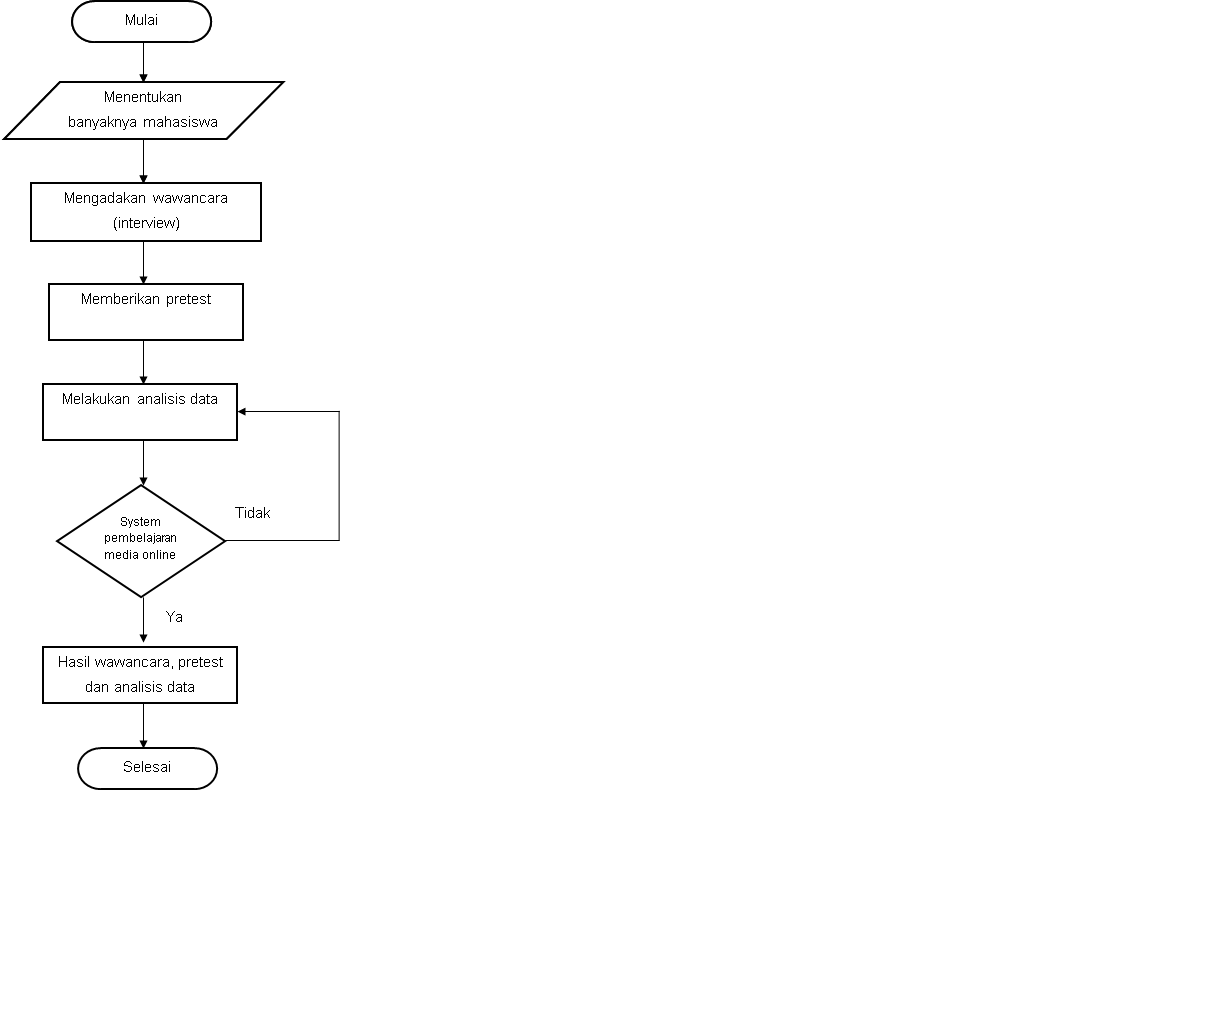
\includegraphics[width=17cm]{gambar/1}
\end{figure}

\section{Jadwal Penelitian}

\begin{center}
Tabel 3.2. Jadwal Penelitian.
\end{center}
\vspace{-0.5cm}
\begin{figure}[ht!]
  \centering
    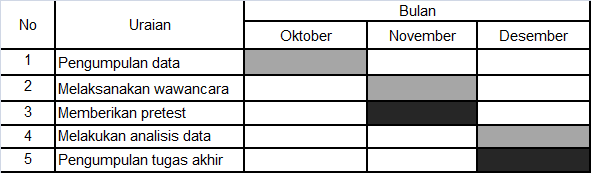
\includegraphics[width=14cm]{gambar/3}
\end{figure}

%-----------------------------------------------------------------
%Disini akhir masukan Bab
%-----------------------------------------------------------------

%-----------------------------------------------------------------
%Disini awal masukan untuk Daftar Pustaka
%-----------------------------------------------------------------
%%\nocite{Abel2010,Guerbas201350}
%%\bibliography{research-plan}
%%\bibliographystyle{plainnat}
\begin{thebibliography}{9}

\bibitem[satu(2013)]{satu01}
berita-21.blogspot.com/2013/07/contoh-proposal-pengajuan-judul-tugas.html

\bibitem[dua(2013)]{dua02}
aifitra.blogdetik.com/index.php/2013/12/25/keuntungan-dan-manfaat-menggunakan-e-learning-bagi-guru-dan-siswa/html

\bibitem[tiga(2013)]{tiga03}
anasuciana.blogspot.com/2013/12/e-learning-sebagai-penunjang.html

\bibitem[empat(2013)]{empat04}
ricaamelia.blogspot.com/2012/03/peranan-pembelajaran-e-learning-dalam.html




\end{thebibliography}
\addcontentsline{toc}{chapter}{DAFTAR PUSTAKA}
%-----------------------------------------------------------------
%Disini akhir masukan Daftar Pustaka
%-----------------------------------------------------------------

\end{document}